\documentclass{article}
\usepackage{graphicx}
\usepackage{subcaption}

\begin{document}

\title{Side-by-Side Graphics Using Subfigure}
\author{SRESTA TEWARI}
\date{\today}
\maketitle

\section{Introduction}
In this document, we demonstrate how to include side-by-side graphics using the subfigure feature from the subcaption package.Here we showcase the different types of beverages through the two different pictures of Tea and Coffee.

\section{TEA VS COFFEE (FIGURES)}

\begin{figure}[h]
    \centering
    \begin{subfigure}[b]{0.45\textwidth}
        \centering
        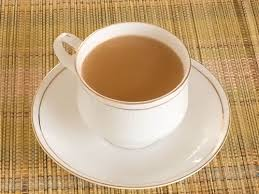
\includegraphics[width=\textwidth]{image1.png} % Replace with your image file
        \caption{First Image}
        \label{fig:first(Tea)}
    \end{subfigure}
    \hfill
    \begin{subfigure}[b]{0.45\textwidth}
        \centering
        
\includegraphics[width=\textwidth]{image2.png} % Replace with your image file
        \caption{Second Image(Coffee)}
        \label{fig:second}
    \end{subfigure}
    \caption{Side by side comparison of two images (HERE TEA AND COFFEE)}
    \label{fig:sidebyside}
\end{figure}
\end{document}